\chapter{Stabilité des systèmes asservis\label{chap-stab}}


\section{Définitions de la stabilité}

\textbf{Un système est dit stable si à une entrée bornée le système produit une sortie bornée}\footnote{Chez 
nos amis anglo-saxons, on rencontre le concept de BIBO (\og bounded input bounded output\fg)}

\textbf{Un système est dit stable lorsque écarté de sa position d'équilibre, il tend à y revenir}

Ces deux définitions sont équivalentes dans le cas des \SLCI. 

\begin{figure}[!h]
    \centering
    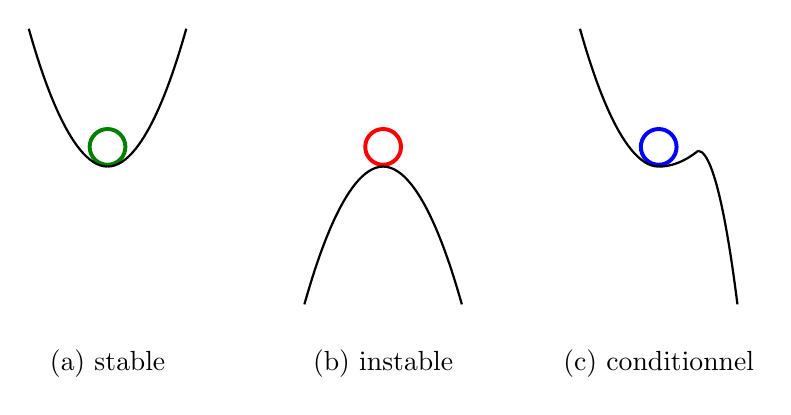
\begin{tikzpicture}
        \draw[green!50!black,line width=0.5mm] (0,0.25) circle (1.5ex);
        \draw[thick] (0,0) parabola (1,1.75) ;
        \draw[thick] (0,0) parabola (-1,1.75) ;
        \node at (0,-2.5) {(a) stable};
        \begin{scope}[xshift=3.5cm]
            \draw[red,line width=0.5mm] (0,0.25) circle (1.5ex);
            \draw[thick] (0,0) parabola (1,-1.75) ;
            \draw[thick] (0,0) parabola (-1,-1.75) ;
            \node at (0,-2.5) {(b) instable};
        \end{scope}
        \begin{scope}[xshift=7cm]
            \draw[blue,line width=0.5mm] (0,0.25) circle (1.5ex);
            \draw[thick] (0,0) parabola (-1,1.75) ;
            \draw[thick] (0,0) parabola (0.5,0.2) ;
            \draw[thick] (0.5,0.2) parabola (1,-1.75) ;
            \node at (0,-2.5) {(c) conditionnel};
        \end{scope}
    \end{tikzpicture}
\caption{Représentation schématique de la stabilité}
\end{figure}

\section{Critère de stabilité}

\begin{criteria}{Condition fondamentale de stabilité}
    \textbf{Un système est stable si sa fonction de transfert ne possède aucun pôles à partie réelle positive.}
\end{criteria}

\clearpage
\thispagestyle{empty}
\begin{landscape}
    \centering
    %\vspace*{\fill}
    \captionsetup{width=1.15\linewidth}
    \begin{figure}[!h]
        \centering
        \begin{tikzpicture}
        \begin{axis}[                                                                                                                     ticks=none,
            width=1.6\textheight,           
            height=\textwidth,    
            axis x line=center,                                                                            
            axis y line=center,
            xmin=-12.5,                                                                                                  
            xmax=12.5,
            ymin=-5,                                                                                                         
            ymax=5,
            xlabel={\LARGE $\Re{(p)}$},
            ylabel={\LARGE $\Im{(p)}$},
            xlabel style={right},
            ylabel style={above},                                                                                       
            ]      
            \draw [white!90!blue,fill=white!95!blue]   (axis cs:-12.5,-5) rectangle (axis cs:0,5);
            \draw [white!90!black,fill=white!90!black] (axis cs:0,-5) rectangle (axis cs:12.5,5);

            \draw [ultra thick,-latex]   (axis cs:-12.5,0) -- (axis cs:12.5,0);
            \draw [ultra thick,-latex]   (axis cs:0,-5) -- (axis cs:0,5);

            \coordinate (pt01) at (axis cs:-6.5,4.5);
            \coordinate (pt02) at (axis cs:6.5,4.5);

            \coordinate (pt1) at (axis cs:-12.5,2.0);
            \addplot[mark=x,black!60!green,ultra thick,only marks,mark size=7pt]  coordinates{ (-11,1.5) (-11,-1.5) } ;      
            \draw[ultra thick,dotted,color=black!60!green] (axis cs:-11,1.5) -- (axis cs:-11,-1.5) ;

            \coordinate (pt2) at (axis cs:-7,1.0);
            \addplot[mark=x,black!10!green,ultra thick,only marks,mark size=7pt]  coordinates{ (-5,0.5) (-5,-0.5) } ;  
            \draw[ultra thick,dotted,color=black!10!green] (axis cs:-5,0.5) -- (axis cs:-5,-0.5) ;

            \coordinate (pt3) at (axis cs:-10.25,-3.0);
            \addplot[mark=x,black!50!red,ultra thick,only marks,mark size=7pt]    coordinates{ (-8,0) } ;             

            \coordinate (pt4) at (axis cs:-4.75,-3.0);
            \addplot[mark=x,red,ultra thick,only marks,mark size=7pt]    coordinates{ (-2,0) } ;                      

            \coordinate (pt5) at  (axis cs:1.25,-5);
            \coordinate (pt52) at (axis cs:1.25,-3);
            \addplot[mark=x,black,ultra thick,only marks,mark size=7pt]  coordinates{ (0,0) } ;                      

            \coordinate (pt6) at (axis cs:1.25,2);
            \coordinate (pt62) at (axis cs:1.25,0);
            \addplot[mark=x,black!50!white,ultra thick,only marks,mark size=7pt]  coordinates{ (0,2) (0,-2) } ;              
            \draw[ultra thick,dotted,color=black!50!white] (axis cs:0,-2) to[bend right] (axis cs:0,2);

            \coordinate (pt7) at (axis cs:8.25,2);
            \addplot[mark=x,blue,ultra thick,only marks,mark size=7pt]   coordinates{ (11,1.5) (11,-1.5) } ;                
            \draw[ultra thick,dotted,color=blue] (axis cs:11,1.5) -- (axis cs:11,-1.5) ;

            \coordinate (pt8) at (axis cs:6.5,-3);
            \addplot[mark=x,orange,ultra thick,only marks,mark size=7pt] coordinates{ (8,0) } ;                  

        \end{axis}


            \node at (pt01) {\textbf{\Large STABLE}};
            \node at (pt02) {\textbf{\Large INSTABLE}};
            % pt1
            \node[anchor=south west] at (pt1) {
                \begin{tikzpicture}
                    \begin{axis}[
                    ticks=none,
                    width=4cm,    
                    height=4cm,    
                    axis x line=center,                                                                            
                    axis y line=center,
                    xmin=-0.5,                                                                                                                    xmax=6.5,
                    ymin=-0.5,                                                                        
                    ymax=2.5,
                    xlabel={$t$},
                    ylabel={$s(t)$},
                    xlabel style={below right},
                    ylabel style={right}
                    ]
                    \addplot [very thick,color=black!60!green,domain=0:10, samples=501,unbounded coords=jump]{1.2*sin(4.5*deg(x))*exp(-0.7*x)};
                    \addplot [thick,dotted,color=black,domain=0:10, samples=501,unbounded coords=jump]{1.2*exp(-0.7*x)+1};
                    \addplot [thick,dotted,color=black,domain=0:10, samples=501,unbounded coords=jump]{-1.2*exp(-0.7*x)+1};
                    \end{axis}
                \end{tikzpicture}
            };

            % pt2
            \node[anchor=south west] at (pt2) {
                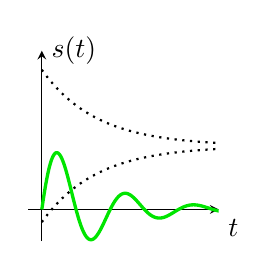
\begin{tikzpicture}
                    \begin{axis}[
                    ticks=none,
                    width=4cm,    
                    height=4cm,    
                    axis x line=center,                                                                            
                    axis y line=center,
                    xmin=-0.5,                                                                                                                    xmax=6.5,
                    ymin=-0.5,                                                                        
                    ymax=2.5,
                    xlabel={$t$},
                    ylabel={$s(t)$},
                    xlabel style={below right},
                    ylabel style={right}
                    ]
                    \addplot [very thick,color=black!10!green,domain=0:10, samples=501,unbounded coords=jump]{1.2*sin(2.5*deg(x))*exp(-0.5*x)};
                    \addplot [thick,dotted,color=black,domain=0:10, samples=501,unbounded coords=jump]{1.2*exp(-0.5*x)+1};
                    \addplot [thick,dotted,color=black,domain=0:10, samples=501,unbounded coords=jump]{-1.2*exp(-0.5*x)+1};
                    \end{axis}
                \end{tikzpicture}
            };
            % pt3
            \node[anchor=south west] at (pt3) {
                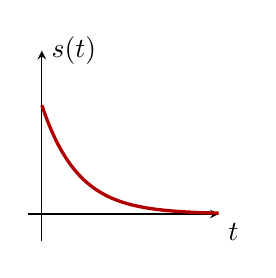
\begin{tikzpicture}
                    \begin{axis}[
                    ticks=none,
                    width=4cm,    
                    height=4cm,    
                    axis x line=center,                                                                            
                    axis y line=center,
                    xmin=-0.5,                                                                                                                    xmax=6.5,
                    ymin=-0.5,                                                                        
                    ymax=3,
                        xlabel={$t$},
                        ylabel={$s(t)$},
                    xlabel style={below right},
                    ylabel style={right}
                    ]
                    \addplot [very thick,color=black!30!red,domain=0:10, samples=501,unbounded coords=jump]{2*exp(-0.75*x)};
                    \end{axis}
                \end{tikzpicture}
            };
            % pt4
            \node[anchor=south west] at (pt4) {
                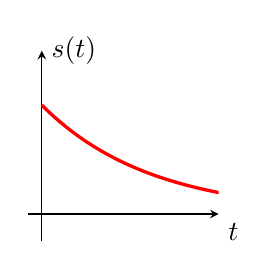
\begin{tikzpicture}
                    \begin{axis}[
                    ticks=none,
                    width=4cm,    
                    height=4cm,    
                    axis x line=center,                                                                            
                    axis y line=center,
                    xmin=-0.5,                                                                                                                    xmax=6.5,
                    ymin=-0.5,                                                                        
                    ymax=3,
                        xlabel={$t$},
                        ylabel={$s(t)$},
                    xlabel style={below right},
                    ylabel style={right}
                    ]
                    \addplot [very thick,color=red,domain=0:10, samples=501,unbounded coords=jump]{2*exp(-0.25*x)};
                    \end{axis}
                \end{tikzpicture}
            };
            % pt5
            \node[anchor=south west] at (pt5) {
                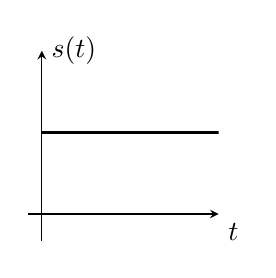
\begin{tikzpicture}
                    \begin{axis}[
                    ticks=none,
                    width=4cm,    
                    height=4cm,    
                    axis x line=center,                                                                            
                    axis y line=center,
                    xmin=-0.5,                                                                                                                    xmax=6.5,
                    ymin=-0.5,                                                                        
                    ymax=3,
                    xlabel={$t$},
                    ylabel={$s(t)$},
                    xlabel style={below right},
                    ylabel style={right}
                    ]
                    \addplot [very thick,color=black,domain=0:10, samples=501,unbounded coords=jump]{1.5};
                    \end{axis}
                \end{tikzpicture}
            };
            % pt52
            \node[anchor=south west] at (pt52) {
                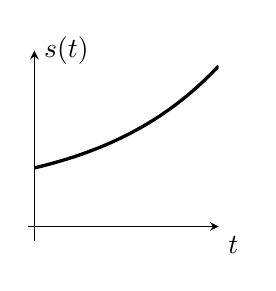
\begin{tikzpicture}
                    \begin{axis}[
                    ticks=none,
                    width=4cm,    
                    height=4cm,    
                    axis x line=center,                                                                            
                    axis y line=center,
                    xmin=-0.5,                                                                                                                    xmax=15,
                    ymin=-0.5,                                                                        
                    ymax=6,
                    xlabel={$t$},
                    ylabel={$s(t)$},
                    xlabel style={below right},
                    ylabel style={right}
                    ]
                    \addplot [very thick,color=black,domain=0:15, samples=501,unbounded coords=jump]{1+exp(0.1*x)};
                    \end{axis}
            \end{tikzpicture}
            };
            % pt6
            \node[anchor=south west] at (pt6) {
                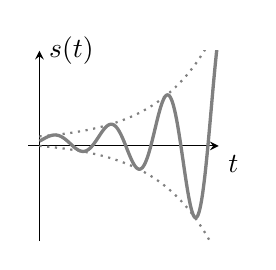
\begin{tikzpicture}
                    \begin{axis}[
                    ticks=none,
                    width=4cm,    
                    height=4cm,    
                    axis x line=center,                                                                            
                    axis y line=center,
                    xmin=-0.5,                                                                                                                    xmax=8,
                    ymin=-20,                                                                        
                    ymax=20,
                    xlabel={$t$},
                    ylabel={$s(t)$},
                    xlabel style={below right},
                    ylabel style={right}
                    ]
              \addplot [very thick,color=black!50!white,domain=0:10, samples=501,unbounded coords=jump]{sin(2.5*deg(x))*exp(0.40*x)+1};
              \addplot [thick,dotted,color=black!50!white,domain=0:10, samples=501,unbounded coords=jump]{ exp(0.4*x)+1};
              \addplot [thick,dotted,color=black!50!white,domain=0:10, samples=501,unbounded coords=jump]{-exp(0.4*x)+1};
                    \end{axis}
                \end{tikzpicture}
            };
            % pt62
            \node[anchor=south west] at (pt62) {
                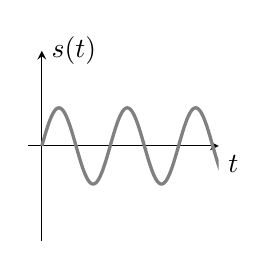
\begin{tikzpicture}
                    \begin{axis}[
                    ticks=none,
                    width=4cm,    
                    height=4cm,    
                    axis x line=center,                                                                            
                    axis y line=center,
                    xmin=-0.5,                                                                                                                    xmax=6.5,
                    ymin=-2.5,                                                                        
                    ymax=2.5,
                    xlabel={$t$},
                    ylabel={$s(t)$},
                    xlabel style={below right},
                    ylabel style={right}
                    ]
                    \addplot [very thick,color=black!50!white,domain=0:10, samples=501,unbounded coords=jump]{sin(2.5*deg(x))};
                    \end{axis}
                \end{tikzpicture}
            };
            % pt7
            \node[anchor=south west] at (pt7) {
                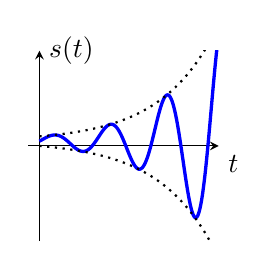
\begin{tikzpicture}
                    \begin{axis}[
                    ticks=none,
                    width=4cm,    
                    height=4cm,    
                    axis x line=center,                                                                            
                    axis y line=center,
                    xmin=-0.5,                                                                                                                    xmax=8.0,
                    ymin=-20,                                                                        
                    ymax=20,
                    xlabel={$t$},
                    ylabel={$s(t)$},
                    xlabel style={below right},
                    ylabel style={right}
                    ]
              \addplot [very thick,color=blue,domain=0:10, samples=501,unbounded coords=jump]{sin(2.5*deg(x))*exp(0.40*x)+1};
              \addplot [thick,dotted,color=black,domain=0:10, samples=501,unbounded coords=jump]{ exp(0.4*x)+1};
              \addplot [thick,dotted,color=black,domain=0:10, samples=501,unbounded coords=jump]{-exp(0.4*x)+1};
                    \end{axis}
              \end{tikzpicture}
            };
            % pt8
            \node[anchor=south west] at (pt8) {
                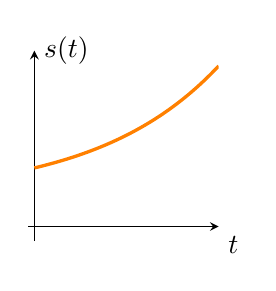
\begin{tikzpicture}
                    \begin{axis}[
                    ticks=none,
                    width=4cm,    
                    height=4cm,    
                    axis x line=center,                                                                            
                    axis y line=center,
                    xmin=-0.5,                                                                                                                    xmax=15,
                    ymin=-0.5,                                                                        
                    ymax=6,
                    xlabel={$t$},
                    ylabel={$s(t)$},
                    xlabel style={below right},
                    ylabel style={right}
                    ]
                    \addplot[very thick,color=orange,domain=0:15,samples=501,unbounded coords=jump]{1+exp(0.1*x)};
                    \end{axis}
                \end{tikzpicture}
            };
        \end{tikzpicture}
    \caption{Stabilité d'un SLCI d'après la carte des pôles de sa fonction de transfert et de leurs
    réponses impulsionnelles.
    (Vert) Deux pôles complexes conjugués. 
    (Rouge) Pôle à partie réel négative. 
    (Gris) Deux pôles complexes conjugués à partie réelle nulle.
    (Noir) Pôle nul.
    (Bleu) Deux pôles complexes conjugués à partie réelle positive.
    (Orange) Pôle à partie réel positive.}
    \end{figure}
%    %\vfill
\end{landscape}

\clearpage
\pagestyle{fancy}
\captionsetup{width=0.8\linewidth}


\paragraph{Inconvénients de la condition fondamentale}

\subsection{Critère algébrique de Routh}

Routh\footnote{Edward John Routh (1831-1907), mathématicien anglais.}
$$
H_{BF}(p)=\dfrac{N(p)}{D(p)}=\dfrac{a_mp^m+a_{m-1}p^{m-1}+\ldots+a_1p+a_0}{b_np^n+b_{n-1}p^{n-1}+\ldots+b_1p+b_0}
$$

l'équation caractéristique :
\begin{align}
    D(p)&=0 \nonumber\\
    b_np^n+b_{n-1}p^{n-1}+\ldots+b_1p+b_0 &= 0
\end{align}

\begin{criteria}{Condition nécessaire (Routh)}
    \textbf{Un système d'ordre $n$ est stable si tous les coefficients ($b_i\forall i\neq n$) 
    de son équation caractéristique sont de même signe que $b_n$.}
\end{criteria}

Cette condition nécessaire s'avère suffisante si le système est du premier ou du second ordre.
Pour un ordre supérieur il faut construire le tableau de Routh à partir des coéfficients de $D(p)$,
pour appliquer un critère suplémentaire. 

\subsubsection{Tableau de Routh}
Dans le cas où la condition nécessaire est respectée et $n>2$, il faut constuire le tableau de Routh à partir 
des coéfficients de l'équation caractéristique de la foction de transfert en boucle fermée.

Le tableau de Routh est constitué de $n$ lignes et de $k$ colonnes où $k=n/2+1$\footnote{On réalise ici une division entière. Par exemple si $n=5$, $k=2+1=3$ et si $n=6$, $k=3+1=4$}. L'élément $A_{ij}$ correspond à l'élément de la $i$-ème ligne et $j$-ème colonne.
\[
\begin{matrix}
    p^n    \\
    p^{n-1}\\
    p^{n-2}\\
    p^{n-3}\\
    \vdots \\
    p^1    \\
    p^0    \\
\end{matrix}
\begin{vmatrix}
    A_{11}     & A_{12}     & A_{13}     & \cdots & A_{1(k-1)}     & A_{1k}      \\
    A_{21}     & A_{22}     & A_{23}     & \cdots & A_{2(k-1)}     & A_{2k}      \\
    A_{31}     & A_{32}     & A_{33}     & \cdots & A_{3(k-1)}     & A_{3k}      \\
    A_{41}     & A_{42}     & A_{43}     & \cdots & A_{4(k-1)}     & A_{4k}      \\
    \vdots     & \vdots     & \vdots     & A_{ij} & \vdots         & \vdots      \\
    A_{(n-1)1} & A_{(n-1)2} & A_{(n-1)3} & \cdots & A_{(n-1)(k-1)} & A_{(n-1)k}  \\
    A_{n1}     & A_{n2}     & A_{n3}     & \cdots & A_{n(k-1)}     & A_{nk}
\end{vmatrix}
\]

Les deux premières lignes du tableau sont directement construites à partir des coéfficients de $D(p)$.
\[
\begin{matrix}
    p^n    \\
    p^{n-1}\\
    \hline
    \vdots \\
\end{matrix}
\begin{vmatrix}
    b_n       & b_{n-2}    & b_{n-4}    & \cdots & b_2            & b_0         \\
    b_{n-1}   & b_{n-3}    & b_{n-5}    & \cdots & b_1            & 0           \\
    \hline
    \vdots    & \vdots     & \vdots     & \vdots & \vdots         & \vdots      \\
    \end{vmatrix}
\]
si $n$ est impaire la dernière colonne de la seconde ligne est non-nulle:
\[
\begin{matrix}
    p^n    \\
    p^{n-1}\\
    \hline
    \vdots \\
\end{matrix}
\begin{vmatrix}
    b_n       & b_{n-2}    & b_{n-4}    & \cdots & b_3            & b_1         \\
    b_{n-1}   & b_{n-3}    & b_{n-5}    & \cdots & b_2            & b_0         \\
    \hline
    \vdots    & \vdots     & \vdots     & \vdots & \vdots         & \vdots      \\
    \end{vmatrix}
\]

Les éléments de la troisième ligne sont construits à partir du 
déterminant\footnote{Nous rappellons le calcul d'un déterminant d'une matrice 
2$\times$2 tel que $\begin{vmatrix} a & b \\ c & d \end{vmatrix}=ad-bc$} d'élements des deux premières lignes.
\[
\begin{matrix}
    p^n    \\
    p^{n-1}\\
    \hline
    p^{n-2}\\
    \vdots \\
\end{matrix}
\begin{vmatrix}
    \textcolor{red}{b_n}       & \textcolor{red}{b_{n-2}}    & b_{n-4}    & \cdots & b_3            & b_1         \\
    \textcolor{red}{b_{n-1}}   & \textcolor{red}{b_{n-3}}    & b_{n-5}    & \cdots & b_2            & b_0         \\
    \hline
    %\hmm{A_{31}}{red}   & A_{32}     & A_{33}     & \cdots & \cdots         & \cdots      \\
    A_{31}  & A_{32}     & A_{33}     & \cdots & \cdots         & \cdots      \\
    \vdots    & \vdots     & \vdots     & \vdots & \vdots         & \vdots      \\
\end{vmatrix}
\Rightarrow
A_{31}=-\dfrac{1}{b_{n-1}}\begin{vmatrix} b_{n}  & b_{n-2} \\ b_{n-1} & b_{n-3}\end{vmatrix}
\]

\[
\begin{matrix}
    p^n    \\
    p^{n-1}\\
    \hline
    p^{n-2}\\
    \vdots \\
\end{matrix}
\begin{vmatrix}
    \textcolor{blue}{b_n}       & b_{n-2}    & \textcolor{blue}{b_{n-4}}    & \cdots & b_3            & b_1         \\
    \textcolor{blue}{b_{n-1}}   & b_{n-3}    & \textcolor{blue}{b_{n-5}}    & \cdots & b_2            & b_0         \\
    \hline
    %A_{31}    & \hmm{A_{32}}{blue}     & A_{33}     & \cdots & \cdots         & \cdots      \\
    A_{31}    & A_{32}     & A_{33}     & \cdots & \cdots         & \cdots      \\
    \vdots    & \vdots     & \vdots     & \vdots & \vdots         & \vdots      \\
\end{vmatrix}
\Rightarrow
A_{32}=-\dfrac{1}{b_{n-1}}\begin{vmatrix} b_{n}  & b_{n-4} \\ b_{n-1} & b_{n-5}\end{vmatrix}
\]

On construit de la même manière la quatrième ligne :
\[
\begin{matrix}
    p^n    \\
    p^{n-1}\\
    \hline
    p^{n-2}\\
    p^{n-3}\\
    \vdots \\
\end{matrix}
\begin{vmatrix}
    b_n       & b_{n-2}    & b_{n-4}    & \cdots & b_3            & b_1         \\
     \textcolor{red}{b_{n-1}}   &  \textcolor{red}{b_{n-3}}    & b_{n-5}    & \cdots & b_2            & b_0         \\
    \hline
     \textcolor{red}{A_{31}}     &  \textcolor{red}{A_{32}}    & A_{33}    & \cdots & \cdots         & \cdots      \\
    %\hmm{A_{41}}{red}      & A_{42}     & A_{43}    & \cdots & \cdots         & \cdots      \\
    A_{41}      & A_{42}     & A_{43}    & \cdots & \cdots         & \cdots      \\
    \vdots    & \vdots     & \vdots     & \vdots & \vdots         & \vdots      \\
    \end{vmatrix}
\Rightarrow
A_{41}=-\dfrac{1}{A_{31}}\begin{vmatrix} A_{21} & A_{22} \\ A_{31} & A_{22} \end{vmatrix}
\]

\[
\begin{matrix}
    p^n    \\
    p^{n-1}\\
    \hline
    p^{n-2}\\
    p^{n-3}\\
    \vdots \\
\end{matrix}
\begin{vmatrix}
    b_n       & b_{n-2}    & b_{n-4}    & \cdots & b_3            & b_1         \\
     \textcolor{blue}{b_{n-1}}   &  b_{n-3}    & \textcolor{blue}{b_{n-5}}    & \cdots & b_2            & b_0         \\
    \hline
     \textcolor{blue}{A_{31}}     &  A_{32}    & \textcolor{blue}{A_{33}}    & \cdots & \cdots         & \cdots      \\
    %A_{41}      & \hmm{A_{42}}{blue}     & A_{43}    & \cdots & \cdots         & \cdots      \\
    A_{41}      & A_{42}     & A_{43}    & \cdots & \cdots         & \cdots      \\
    \vdots    & \vdots     & \vdots     & \vdots & \vdots         & \vdots      \\
    \end{vmatrix}
\Rightarrow
A_{42}=-\dfrac{1}{A_{31}}\begin{vmatrix} A_{21} & A_{23} \\ A_{31} & A_{33} \end{vmatrix}
\]

Et ainsi de suite jusque la dernière ligne du tableau. 

\newpage
La formule générale pour obtenir l'élément $A_{ij}$ est alors :

\begin{bequation}[ams align]
A_{ij}=-\dfrac{1}{A_{(i-1)1}}\begin{vmatrix} A_{(i-2)1} & A_{(i-2)(j+1)} \\ A_{(i-1)1} & A_{(i-1)(j+1)} \end{vmatrix}
\end{bequation}

\newcommand*{\DoTikzmarkU}[1]{%
\tikzset{external/export next=false}
    \tikz[remember picture] \coordinate[shift={(-1ex,1.75ex)}](#1);%
}
\newcommand*{\DoTikzmarkD}[1]{%
\tikzset{external/export next=false}
    \tikz[remember picture] \coordinate[shift={(-1ex,-10ex)}](#1);%
}

\newcommand*{\colrow}[3][]{%
\tikzset{external/export next=false}
  \tikz[overlay,remember picture, line width=40pt]
    \draw[shorten >=-1.25em, shorten <=-.5em, #1] (#2.north)--(#3.north);
}                                                                                                                             

Le critère s'applique sur la première colonne (dite des pivots) du tableau de Routh ainsi construit. 
\[
\begin{matrix}
    p^n    \\
    p^{n-1}\\
    p^{n-2}\\
    p^{n-3}\\
    \vdots \\
    p^1    \\
    p^0    \\
\end{matrix}
\begin{vmatrix}
    b_n\DoTikzmarkU{num-1}  & b_{n-2}    & b_{n-4}    & \cdots & b_2        & b_0         \\
    b_{n-1}                 & b_{n-3}    & b_{n-5}    & \cdots & b_1        & 0           \\
    A_{31}                  & A_{32}     & A_{33}     & \cdots & A_{3(k-1)} & 0           \\
    A_{41}                  & A_{42}     & A_{43}     & \cdots & 0          & 0           \\
    \vdots                  & \vdots     & \vdots     & \vdots & \vdots     & 0           \\
    A_{(n-1)1}              & A_{(n-1)2} & 0          & \cdots & 0          & 0           \\
    b_0\DoTikzmarkU{num-2}  & 0          & 0          & \cdots & 0          & 0
\end{vmatrix}
\]
\colrow[green,opacity=.2]{num-1}{num-2}

\begin{criteria}{Critère de Routh}
    \textbf{Un système est stable si tous les termes de la colonne des pivots du tableau de Routh sont de même signes.}
\end{criteria}

\paragraph{Remarques:}
Le nombre de changement de signe, nous donne le nombre de pôles à partie réelle de la fonction de transfert en boucle fermée.

\subsubsection{Exemple}

Soit un système asservi caractérisé par le schéma-bloc suivant:

\begin{center}
    \begin{tikzpicture}
        \sbEntree{E}
        \sbComp[5.0]{comp}{E}
        \sbRelier[$E(p)$]{E}{comp}
        \sbBloc[1.5]{B}{$H(p)=\dfrac{K}{p(p^2+p+3)}$}{comp}
        \sbRelier[$\epsilon$]{comp}{B}
        \sbSortie[5.0]{S}{B}
        \sbRelier[$S(p)$]{B}{S}
    \sbRenvoi{B-S}{comp}{}
\end{tikzpicture}
\end{center}

La fonction de transfert en boucle fermée $H_{BF}$ s'écrit :
$$
H_{BF}=\dfrac{H(p)}{1+H(p)}=\dfrac{K}{p^3+p^2+3p+K}.
$$

L'équation caractéristique $D(p)$ de $H_{BF}$ est donc 
$$
D(p)=p^3+p^2+3p+K,
$$
Nous constatons que le système est d'ordre 3 dont les coefficients sont :
\begin{align*}
    b_3&=1\\
    b_2&=1\\
    b_1&=3\\
    b_0&=K\\
\end{align*}
Le critère nécessaire de Routh est donc respecté pour $K>0$.


Construisons maintenant le tableau de Routh:

\[
\begin{matrix}
    p^3 \\
    p^2 \\
    \hline
    p^1 \\
    p^0 \\
\end{matrix}
\begin{vmatrix}
     1      & 3  \\
     1      & K  \\
    \hline
    A_{31}  & 0  \\
    A_{41}  & 0    
    \end{vmatrix}
\]

$$
A_{31}=-\begin{vmatrix}1 & 3 \\ 1 & K\end{vmatrix}=3-K
$$

$$
A_{41}=-\dfrac{1}{A_{31}}\begin{vmatrix} 1 & K \\ A_{31} & 0 \end{vmatrix}=K
$$
\renewcommand*{\DoTikzmarkU}[1]{%
\tikzset{external/export next=false}
    \tikz[remember picture] \coordinate[shift={(-0.5ex,1.75ex)}](#1);%
}
\renewcommand*{\DoTikzmarkD}[1]{% 
\tikzset{external/export next=false}
    \tikz[remember picture] \coordinate[shift={(-0.5ex,-6ex)}](#1);%
}
\renewcommand*{\colrow}[3][]{%
\tikzset{external/export next=false}
  \tikz[overlay,remember picture, line width=30pt]
  \draw[shorten >=-.5em, shorten <=-.5em, #1] (#2.north)--(#3.north);
}
\[
\begin{matrix}
    p^3 \\
    p^2 \\
   % \hline
    p^1 \\
    p^0 \\
\end{matrix}
\begin{vmatrix}
    1\DoTikzmarkU{num-3}     & 3  \\
    1\DoTikzmarkD{num-4}     & K  \\
   % \hline
    3-K                      & 0  \\
    K                        & 0    
    \end{vmatrix}
\]
\colrow[green,opacity=.2]{num-3}{num-4}

La colonne des pivots sont tous de même signe si $3-K>0$ et $K>0$ (déjà établie par la condition nécessaire de Routh).
La condition sur $K$ pour que le système soit stable est donc :
$$
0<K<3
$$

\subsection{Critère graphique du revers}

Routh s'applique sur la fonction de transfert en boucle fermée, les critères graphiques permettent 
d'étudier la stabilité du système en boucle ouverte.

En effet si l'on considère la boucle de contre réaction unitaire pour l'asservissement d'un système
de fonction de transfert $H(p)$, telle que : 
\begin{center}
    \begin{tikzpicture}
    \sbEntree{E}
    \sbComp[5.0]{comp}{E}
        \sbRelier[$E(p)$]{E}{comp}
        \sbBloc[1.5]{B}{$H(p)$}{comp}
        \sbRelier[$\epsilon$]{comp}{B}
        \sbSortie[5.0]{S}{B}
        \sbRelier[$S(p)$]{B}{S}
    \sbRenvoi{B-S}{comp}{}
\end{tikzpicture}
\end{center}

la fonction de transfert en boucle ouverte $H_{BO}(p)$ est simplement donné par $H(p)$, et comme nous l'avons 
déjà rencontré à plusieurs occasions, la fonction de transfert en boucle fermée $H_{BF}$ est égale à 
$$
H_{BF}(p)=\dfrac{N(p)}{D(p)}=\dfrac{H_{BO}(p)}{1+H_{BO}(p)},
$$
ainsi étudier les pôles de l'équation caractéristique $D(p)=0$ est équivalent à étudier l'équation 
$$
1+H_{BO}(p)=0\Leftrightarrow H_{BO}(p)=-1
$$
Il est alors possible d'étudier la fonction de transfert en boucle ouverte par rapport au point critique du plan complexe 
$(-1,0)$

\subsubsection{Critère du revers de Nyquist}

\begin{criteria}{Critère du revers (Nyquist)}
\textbf{Un système est stable en boucle fermée si lorsque parcourant 
        le lieu de Nyquist de la boucle ouverte dans le sens des 
        pulsations croissantes, on laisse le point critique sur la gauche.}
\end{criteria}

\begin{figure}[!h]
\begin{center}
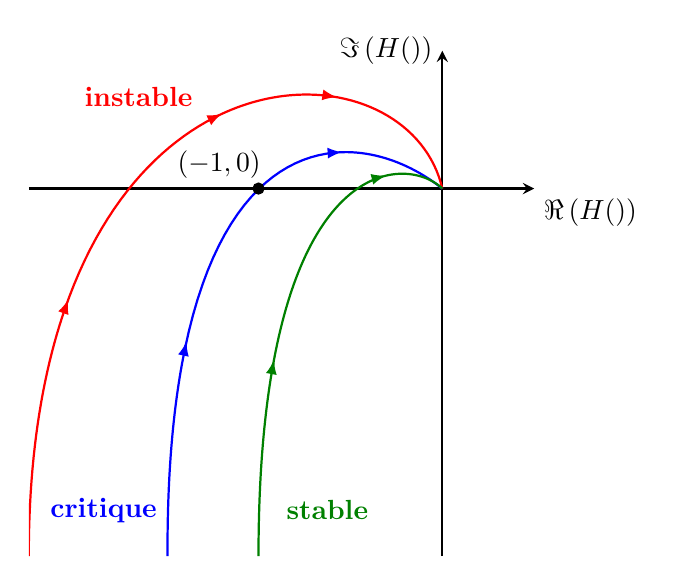
\begin{tikzpicture}
\begin{axis}
    [
    height=8cm,
    width=8cm,
    axis lines = center,
    ticks=none,
    axis line style = thick,
    enlargelimits=false,
    xlabel=$\Re\left(H(\jw)\right)$,
    ylabel=$\Im\left(H(\jw)\right)$,
    xlabel style={below right},
    ylabel style={left},
    ymin=-4,
    ymax=1.5,
    xmin=-2.25,
    xmax=0.5
    ]     
    \addplot [black, mark = *] coordinates {( -1, 0)} {};
    \node [above left,xshift=1ex]  at (axis cs:  -1, 0)   {$(-1,0)$};                
    
    % instable
    \def\xu{-0.2}
    \def\yu{1.75}
    \def\xd{-2.25}
    \def\yd{1.75}
    \def\xt{-2.25}
    \def\yt{-4}
    \addplot [-latex,red,thick,domain=1:0.8,samples=25]
    ({(1-x)*((1-x)*(x*\xu)+x*((1-x)*\xu+x*\xd))+x*((1-x)*((1-x)*\xu+x*\xd)+x*((1-x)*\xd+x*\xt))},
    {(1-x)*((1-x)*(x*\yu)+x*((1-x)*\yu+x*\yd))+x*((1-x)*((1-x)*\yu+x*\yd)+x*((1-x)*\yd+x*\yt))});
    \addplot [-latex,red,thick,domain=0.81:0.5,samples=25]
    ({(1-x)*((1-x)*(x*\xu)+x*((1-x)*\xu+x*\xd))+x*((1-x)*((1-x)*\xu+x*\xd)+x*((1-x)*\xd+x*\xt))},
    {(1-x)*((1-x)*(x*\yu)+x*((1-x)*\yu+x*\yd))+x*((1-x)*((1-x)*\yu+x*\yd)+x*((1-x)*\yd+x*\yt))});
    \addplot [-latex,red,thick,domain=0.51:0.3,samples=25]
    ({(1-x)*((1-x)*(x*\xu)+x*((1-x)*\xu+x*\xd))+x*((1-x)*((1-x)*\xu+x*\xd)+x*((1-x)*\xd+x*\xt))},
    {(1-x)*((1-x)*(x*\yu)+x*((1-x)*\yu+x*\yd))+x*((1-x)*((1-x)*\yu+x*\yd)+x*((1-x)*\yd+x*\yt))});
    \addplot [red,thick,domain=0.31:0,samples=25]
    ({(1-x)*((1-x)*(x*\xu)+x*((1-x)*\xu+x*\xd))+x*((1-x)*((1-x)*\xu+x*\xd)+x*((1-x)*\xd+x*\xt))},
    {(1-x)*((1-x)*(x*\yu)+x*((1-x)*\yu+x*\yd))+x*((1-x)*((1-x)*\yu+x*\yd)+x*((1-x)*\yd+x*\yt))});

    \node [red,right]  at (axis cs:  -2, 1.0)   {\textbf{instable}};                

    % critique 
    \def\xu{-0.5}
    \def\yu{0.8}
    \def\xd{-1.506}
    \def\yd{0.8}
    \def\xt{-1.495}
    \def\yt{-4}
    \addplot [-latex,blue,thick,domain=1:0.8,samples=50]
    ({(1-x)*((1-x)*(x*\xu)+x*((1-x)*\xu+x*\xd))+x*((1-x)*((1-x)*\xu+x*\xd)+x*((1-x)*\xd+x*\xt))},
    {(1-x)*((1-x)*(x*\yu)+x*((1-x)*\yu+x*\yd))+x*((1-x)*((1-x)*\yu+x*\yd)+x*((1-x)*\yd+x*\yt))});
    \addplot [-latex,blue,thick,domain=0.81:0.3,samples=25]
    ({(1-x)*((1-x)*(x*\xu)+x*((1-x)*\xu+x*\xd))+x*((1-x)*((1-x)*\xu+x*\xd)+x*((1-x)*\xd+x*\xt))},
    {(1-x)*((1-x)*(x*\yu)+x*((1-x)*\yu+x*\yd))+x*((1-x)*((1-x)*\yu+x*\yd)+x*((1-x)*\yd+x*\yt))});
    \addplot [blue,thick,domain=0.31:0,samples=25]
    ({(1-x)*((1-x)*(x*\xu)+x*((1-x)*\xu+x*\xd))+x*((1-x)*((1-x)*\xu+x*\xd)+x*((1-x)*\xd+x*\xt))},
    {(1-x)*((1-x)*(x*\yu)+x*((1-x)*\yu+x*\yd))+x*((1-x)*((1-x)*\yu+x*\yd)+x*((1-x)*\yd+x*\yt))});
    \node [blue,left]  at (axis cs:  -1.5, -3.5)   {\textbf{critique}};                

    %stable
    \def\xu{-0.206}
    \def\yu{0.4}
    \def\xd{-1}
    \def\yd{0.38}
    \def\xt{-1}
    \def\yt{-4}
    \addplot [-latex,green!50!black,thick,domain=1:0.8,samples=50]
    ({(1-x)*((1-x)*(x*\xu)+x*((1-x)*\xu+x*\xd))+x*((1-x)*((1-x)*\xu+x*\xd)+x*((1-x)*\xd+x*\xt))},
    {(1-x)*((1-x)*(x*\yu)+x*((1-x)*\yu+x*\yd))+x*((1-x)*((1-x)*\yu+x*\yd)+x*((1-x)*\yd+x*\yt))});
    \addplot [-latex,green!50!black,thick,domain=0.81:0.3,samples=50]
    ({(1-x)*((1-x)*(x*\xu)+x*((1-x)*\xu+x*\xd))+x*((1-x)*((1-x)*\xu+x*\xd)+x*((1-x)*\xd+x*\xt))},
    {(1-x)*((1-x)*(x*\yu)+x*((1-x)*\yu+x*\yd))+x*((1-x)*((1-x)*\yu+x*\yd)+x*((1-x)*\yd+x*\yt))});
    \addplot [color=green!50!black,thick,domain=0.31:0,samples=50]
    ({(1-x)*((1-x)*(x*\xu)+x*((1-x)*\xu+x*\xd))+x*((1-x)*((1-x)*\xu+x*\xd)+x*((1-x)*\xd+x*\xt))},
    {(1-x)*((1-x)*(x*\yu)+x*((1-x)*\yu+x*\yd))+x*((1-x)*((1-x)*\yu+x*\yd)+x*((1-x)*\yd+x*\yt))});

    \node [green!50!black,right]  at (axis cs:  -0.9, -3.5)   {\textbf{stable}};                
\end{axis}
\end{tikzpicture}
\end{center}
\caption{Représentation schématique de lieux de Nyquist de trois systèmes: stable, critique et instable vérifiant le critère du revers.
\label{fig-nyquist_revers}}
\end{figure}



% (1-x)*((1-x)*(x*\x1)+x*((1-x)*\x1+x*\x2))+x*((1-x)*((1-x)*\x1+x*\x2)+x*((1-x)*\x2+x*\x3)),
% (1-x)*((1-x)*(x*\y1)+x*((1-x)*\y1+x*\y2))+x*((1-x)*((1-x)*\y1+x*\y2)+x*((1-x)*\y2+x*\y3))


\subsubsection{Critère du revers de Black}
\subsubsection{Critère du revers de Bode}


\subsection{Critère de Nyquist}

Le critère de Nyquist est également un critère graphique mais 
est plus générale que le critère du revers. Il s'appuie sur le 
principe de l'argument de Cauchy\footnote{Nous ne donnerons qu'une présentation élémentaire et sans démonstration
de ce théorème. Un cours d'analyse complexe permettra de compléter cette présentation. On trouvera dans \cite{laas_pc7bis}, 
une introduction plus détaillée ainsi qu'une bibliographie très fournie sur le sujet.}.

\paragraph{Théorème du principe de l'argument de Cauchy}

\begin{figure}[!h]
\begin{center}
\begin{tikzpicture}
\begin{axis}
    [
    name=nyy1,
    height=8cm,
    width=8cm,
    axis lines = center,
    ticks=none,
    axis line style = thick,
    enlargelimits=false,
    xlabel=$\Re\left(p\right)$,
    ylabel=$\Im\left(p\right)$,
    xlabel style={below},
    ylabel style={left},
    ymin=-4,
    ymax=4,
    xmin=-8,
    xmax=8
    ]     
    \pgfmathsetseed{3}
    \draw [decoration={markings, 
           mark=at position 0.2 with {\arrow[line width=2pt]{latex}}},
           postaction={decorate},
           thick,
           red,
           smooth cycle,
           samples=11,
           domain={11:1},
           xshift=3cm,
           yshift=3cm] plot (\x*360/11+5*rnd:1.25cm+0.75cm*rnd) ;
    \node[red] (ct) at (axis cs:-4,2) {\Large$\mathcal{C}$};
    \addplot[mark=x,ultra thick,only marks,mark size=5pt] coordinates{ (-3.0,-0.5) (-6,-1)};
    \addplot[mark=o,ultra thick,only marks,mark size=5pt] coordinates{ (1,0) (-1,1.2) (-2.1,-1.7) };
\end{axis}
\begin{axis}
    [
    at={(nyy1.south east)},xshift=4ex,
    height=8cm,
    width=8cm,
    axis lines = center,
    ticks=none,
    axis line style = thick,
    enlargelimits=false,
    xlabel=$\Re\left(F(p)\right)$,
    ylabel=$\Im\left(F(p)\right)$,
    xlabel style={below},
    ylabel style={left},
    ymin=-4,
    ymax=4,
    xmin=-4,
    xmax=4
    ]     
    \def\m{1.0}
    \def\n{2.1}
    \addplot[decoration={markings,mark=at position 0.1 with {\arrow[line width=2pt]{latex}}},
    postaction={decorate},
    blue,
    thick,
    domain=1:3,
    samples=50,
    smooth cycle] coordinates 
    {(1.9,-1.5) (0,-2) (-0.75,0.35) (0.25,1.25) (1,0.25) (-0.25,-0.75) 
    (-1.1,-1.25) (-1.5,-1) (-2,0) (-1.5,1.5)  (0,2)  (0.75,1.9) (2,0)}; 
    \node[blue] (ct) at (axis cs:-2.5,2) {\Large$\Gamma:F(\mathcal{C})$};
\end{axis}
\end{tikzpicture}
\end{center}
    \caption{Représentation de la transformation d'un contour $\mathcal{C}$ en son image par une fonction analytique $F(p)$
    \label{fig-contour_cauchy}}
\end{figure}

\begin{theorem}{Principe de l'argument de Cauchy} 
    Si un contour $\mathcal{C}$ contient $Z$ zéros et $P$ pôles d'une fonction analytique $F(p)$ 
    sans en traverser aucun, alors quand on le parcourt dans le sens anti-trigonométrique, le contour $\Gamma=F(\mathcal{C})$ 
    fait un nombre de tours autour de l'origine dans le sens trigonométrique égal à,
    $$
    N=Z-P
    $$
\end{theorem}
